\documentclass[twoside]{book}

% Packages required by doxygen
\usepackage{fixltx2e}
\usepackage{calc}
\usepackage{doxygen}
\usepackage[export]{adjustbox} % also loads graphicx
\usepackage{graphicx}
\usepackage[utf8]{inputenc}
\usepackage{makeidx}
\usepackage{multicol}
\usepackage{multirow}
\PassOptionsToPackage{warn}{textcomp}
\usepackage{textcomp}
\usepackage[nointegrals]{wasysym}
\usepackage[table]{xcolor}

% Font selection
\usepackage[T1]{fontenc}
\usepackage[scaled=.90]{helvet}
\usepackage{courier}
\usepackage{amssymb}
\usepackage{sectsty}
\renewcommand{\familydefault}{\sfdefault}
\allsectionsfont{%
  \fontseries{bc}\selectfont%
  \color{darkgray}%
}
\renewcommand{\DoxyLabelFont}{%
  \fontseries{bc}\selectfont%
  \color{darkgray}%
}
\newcommand{\+}{\discretionary{\mbox{\scriptsize$\hookleftarrow$}}{}{}}

% Page & text layout
\usepackage{geometry}
\geometry{%
  a4paper,%
  top=2.5cm,%
  bottom=2.5cm,%
  left=2.5cm,%
  right=2.5cm%
}
\tolerance=750
\hfuzz=15pt
\hbadness=750
\setlength{\emergencystretch}{15pt}
\setlength{\parindent}{0cm}
\setlength{\parskip}{3ex plus 2ex minus 2ex}
\makeatletter
\renewcommand{\paragraph}{%
  \@startsection{paragraph}{4}{0ex}{-1.0ex}{1.0ex}{%
    \normalfont\normalsize\bfseries\SS@parafont%
  }%
}
\renewcommand{\subparagraph}{%
  \@startsection{subparagraph}{5}{0ex}{-1.0ex}{1.0ex}{%
    \normalfont\normalsize\bfseries\SS@subparafont%
  }%
}
\makeatother

% Headers & footers
\usepackage{fancyhdr}
\pagestyle{fancyplain}
\fancyhead[LE]{\fancyplain{}{\bfseries\thepage}}
\fancyhead[CE]{\fancyplain{}{}}
\fancyhead[RE]{\fancyplain{}{\bfseries\leftmark}}
\fancyhead[LO]{\fancyplain{}{\bfseries\rightmark}}
\fancyhead[CO]{\fancyplain{}{}}
\fancyhead[RO]{\fancyplain{}{\bfseries\thepage}}
\fancyfoot[LE]{\fancyplain{}{}}
\fancyfoot[CE]{\fancyplain{}{}}
\fancyfoot[RE]{\fancyplain{}{\bfseries\scriptsize Generated by Doxygen }}
\fancyfoot[LO]{\fancyplain{}{\bfseries\scriptsize Generated by Doxygen }}
\fancyfoot[CO]{\fancyplain{}{}}
\fancyfoot[RO]{\fancyplain{}{}}
\renewcommand{\footrulewidth}{0.4pt}
\renewcommand{\chaptermark}[1]{%
  \markboth{#1}{}%
}
\renewcommand{\sectionmark}[1]{%
  \markright{\thesection\ #1}%
}

% Indices & bibliography
\usepackage{natbib}
\usepackage[titles]{tocloft}
\setcounter{tocdepth}{3}
\setcounter{secnumdepth}{5}
\makeindex

% Hyperlinks (required, but should be loaded last)
\usepackage{ifpdf}
\ifpdf
  \usepackage[pdftex,pagebackref=true]{hyperref}
\else
  \usepackage[ps2pdf,pagebackref=true]{hyperref}
\fi
\hypersetup{%
  colorlinks=true,%
  linkcolor=blue,%
  citecolor=blue,%
  unicode%
}

% Custom commands
\newcommand{\clearemptydoublepage}{%
  \newpage{\pagestyle{empty}\cleardoublepage}%
}

\usepackage{caption}
\captionsetup{labelsep=space,justification=centering,font={bf},singlelinecheck=off,skip=4pt,position=top}

%===== C O N T E N T S =====

\begin{document}

% Titlepage & ToC
\hypersetup{pageanchor=false,
             bookmarksnumbered=true,
             pdfencoding=unicode
            }
\pagenumbering{roman}
\begin{titlepage}
\vspace*{7cm}
\begin{center}%
{\Large P\+A03 }\\
\vspace*{1cm}
{\large Generated by Doxygen 1.8.11}\\
\end{center}
\end{titlepage}
\clearemptydoublepage
\tableofcontents
\clearemptydoublepage
\pagenumbering{arabic}
\hypersetup{pageanchor=true}

%--- Begin generated contents ---
\chapter{Class Index}
\section{Class List}
Here are the classes, structs, unions and interfaces with brief descriptions\+:\begin{DoxyCompactList}
\item\contentsline{section}{\hyperlink{class_a_b_event_queue}{A\+B\+Event\+Queue} \\*An Array-\/\+Based \hyperlink{struct_event}{Event} Queue }{\pageref{class_a_b_event_queue}}{}
\item\contentsline{section}{\hyperlink{struct_event}{Event} }{\pageref{struct_event}}{}
\item\contentsline{section}{\hyperlink{class_event_queue}{Event\+Queue} }{\pageref{class_event_queue}}{}
\item\contentsline{section}{\hyperlink{struct_l_l_e_q_node}{L\+L\+E\+Q\+Node} \\*A node in an \hyperlink{class_l_l_event_queue}{L\+L\+Event\+Queue} }{\pageref{struct_l_l_e_q_node}}{}
\item\contentsline{section}{\hyperlink{class_l_l_event_queue}{L\+L\+Event\+Queue} \\*A Linked-\/\+List-\/\+Based \hyperlink{struct_event}{Event} Queue }{\pageref{class_l_l_event_queue}}{}
\item\contentsline{section}{\hyperlink{class_teller}{Teller} \\*Models a bank teller }{\pageref{class_teller}}{}
\item\contentsline{section}{\hyperlink{class_teller_setup}{Teller\+Setup} }{\pageref{class_teller_setup}}{}
\item\contentsline{section}{\hyperlink{class_teller_setup__1_qn_t}{Teller\+Setup\+\_\+1\+QnT} }{\pageref{class_teller_setup__1_qn_t}}{}
\item\contentsline{section}{\hyperlink{class_teller_setup__n_qn_t}{Teller\+Setup\+\_\+n\+QnT} }{\pageref{class_teller_setup__n_qn_t}}{}
\item\contentsline{section}{\hyperlink{class_tickable}{Tickable} \\*A \hyperlink{class_tickable}{Tickable} object }{\pageref{class_tickable}}{}
\item\contentsline{section}{\hyperlink{class_tickable_queue}{Tickable\+Queue} \\*An \hyperlink{class_event_queue}{Event\+Queue} wrapper that enables tick functionality }{\pageref{class_tickable_queue}}{}
\end{DoxyCompactList}

\chapter{File Index}
\section{File List}
Here is a list of all documented files with brief descriptions\+:\begin{DoxyCompactList}
\item\contentsline{section}{\hyperlink{PA02_8cpp}{P\+A02.\+cpp} \\*Implements the program entry point }{\pageref{PA02_8cpp}}{}
\end{DoxyCompactList}

\chapter{Class Documentation}
\hypertarget{class_city_node_v1}{}\section{City\+Node\+V1 Class Reference}
\label{class_city_node_v1}\index{City\+Node\+V1@{City\+Node\+V1}}


Represents a v1 node in the city adjacency map.  




{\ttfamily \#include $<$Flight\+Map.\+v1.\+h$>$}

\subsection*{Public Member Functions}
\begin{DoxyCompactItemize}
\item 
\hyperlink{class_city_node_v1_abbbcf07a0ef873b9cd4a7c4acc904bfa}{City\+Node\+V1} (const std\+::string \&\hyperlink{class_city_node_v1_aadf0c50a4e35c15a8e13b51afefbdbc5}{name})
\begin{DoxyCompactList}\small\item\em Initializes node with the given name. \end{DoxyCompactList}\item 
\hyperlink{class_city_node_v1_a422f2c8818000e84e4eea3e2ab4028aa}{City\+Node\+V1} ()
\begin{DoxyCompactList}\small\item\em Initializes node with empty name. \end{DoxyCompactList}\end{DoxyCompactItemize}
\subsection*{Public Attributes}
\begin{DoxyCompactItemize}
\item 
std\+::string \hyperlink{class_city_node_v1_aadf0c50a4e35c15a8e13b51afefbdbc5}{name}
\item 
std\+::vector$<$ \hyperlink{struct_connection_v1}{Connection\+V1} $>$ \hyperlink{class_city_node_v1_a32793af0a49d5a187d88a1633f53b5c4}{connections}
\item 
bool \hyperlink{class_city_node_v1_adc01d952c831f5f740674e06940c4844}{visited}
\end{DoxyCompactItemize}


\subsection{Detailed Description}
Represents a v1 node in the city adjacency map. 

\subsection{Constructor \& Destructor Documentation}
\index{City\+Node\+V1@{City\+Node\+V1}!City\+Node\+V1@{City\+Node\+V1}}
\index{City\+Node\+V1@{City\+Node\+V1}!City\+Node\+V1@{City\+Node\+V1}}
\subsubsection[{\texorpdfstring{City\+Node\+V1(const std\+::string \&name)}{CityNodeV1(const std::string &name)}}]{\setlength{\rightskip}{0pt plus 5cm}City\+Node\+V1\+::\+City\+Node\+V1 (
\begin{DoxyParamCaption}
\item[{const std\+::string \&}]{name}
\end{DoxyParamCaption}
)}\hypertarget{class_city_node_v1_abbbcf07a0ef873b9cd4a7c4acc904bfa}{}\label{class_city_node_v1_abbbcf07a0ef873b9cd4a7c4acc904bfa}


Initializes node with the given name. 


\begin{DoxyParams}{Parameters}
{\em name} & The name of the city. \\
\hline
\end{DoxyParams}
\index{City\+Node\+V1@{City\+Node\+V1}!City\+Node\+V1@{City\+Node\+V1}}
\index{City\+Node\+V1@{City\+Node\+V1}!City\+Node\+V1@{City\+Node\+V1}}
\subsubsection[{\texorpdfstring{City\+Node\+V1()}{CityNodeV1()}}]{\setlength{\rightskip}{0pt plus 5cm}City\+Node\+V1\+::\+City\+Node\+V1 (
\begin{DoxyParamCaption}
{}
\end{DoxyParamCaption}
)}\hypertarget{class_city_node_v1_a422f2c8818000e84e4eea3e2ab4028aa}{}\label{class_city_node_v1_a422f2c8818000e84e4eea3e2ab4028aa}


Initializes node with empty name. 

\begin{DoxyNote}{Note}
Required for std\+::map compatibility. 
\end{DoxyNote}


\subsection{Member Data Documentation}
\index{City\+Node\+V1@{City\+Node\+V1}!connections@{connections}}
\index{connections@{connections}!City\+Node\+V1@{City\+Node\+V1}}
\subsubsection[{\texorpdfstring{connections}{connections}}]{\setlength{\rightskip}{0pt plus 5cm}std\+::vector$<${\bf Connection\+V1}$>$ City\+Node\+V1\+::connections}\hypertarget{class_city_node_v1_a32793af0a49d5a187d88a1633f53b5c4}{}\label{class_city_node_v1_a32793af0a49d5a187d88a1633f53b5c4}
\index{City\+Node\+V1@{City\+Node\+V1}!name@{name}}
\index{name@{name}!City\+Node\+V1@{City\+Node\+V1}}
\subsubsection[{\texorpdfstring{name}{name}}]{\setlength{\rightskip}{0pt plus 5cm}std\+::string City\+Node\+V1\+::name}\hypertarget{class_city_node_v1_aadf0c50a4e35c15a8e13b51afefbdbc5}{}\label{class_city_node_v1_aadf0c50a4e35c15a8e13b51afefbdbc5}
\index{City\+Node\+V1@{City\+Node\+V1}!visited@{visited}}
\index{visited@{visited}!City\+Node\+V1@{City\+Node\+V1}}
\subsubsection[{\texorpdfstring{visited}{visited}}]{\setlength{\rightskip}{0pt plus 5cm}bool City\+Node\+V1\+::visited}\hypertarget{class_city_node_v1_adc01d952c831f5f740674e06940c4844}{}\label{class_city_node_v1_adc01d952c831f5f740674e06940c4844}


The documentation for this class was generated from the following files\+:\begin{DoxyCompactItemize}
\item 
\hyperlink{_flight_map_8v1_8h}{Flight\+Map.\+v1.\+h}\item 
\hyperlink{_flight_map_8v1_8cpp}{Flight\+Map.\+v1.\+cpp}\item 
\hyperlink{_flight_map_8v2_8cpp_8cpp}{Flight\+Map.\+v2.\+cpp.\+cpp}\end{DoxyCompactItemize}

\hypertarget{class_city_node_v2}{}\section{City\+Node\+V2 Class Reference}
\label{class_city_node_v2}\index{City\+Node\+V2@{City\+Node\+V2}}


Represents a v2 node in the city adjacency map.  




{\ttfamily \#include $<$Flight\+Map.\+v2.\+h$>$}

\subsection*{Public Member Functions}
\begin{DoxyCompactItemize}
\item 
\hyperlink{class_city_node_v2_ae1f0eb6340a8b885f89376339ec90314}{City\+Node\+V2} (const std\+::string \&\hyperlink{class_city_node_v2_a3cf01413b0ca939d0811ab649981d4a5}{name})
\begin{DoxyCompactList}\small\item\em Initializes node with the given name. \end{DoxyCompactList}\item 
\hyperlink{class_city_node_v2_a73000f4890545ab24a6ba02e609a79a3}{City\+Node\+V2} ()
\begin{DoxyCompactList}\small\item\em Initializes node with empty name. \end{DoxyCompactList}\end{DoxyCompactItemize}
\subsection*{Public Attributes}
\begin{DoxyCompactItemize}
\item 
std\+::string \hyperlink{class_city_node_v2_a3cf01413b0ca939d0811ab649981d4a5}{name}
\item 
std\+::vector$<$ \hyperlink{struct_connection_v2}{Connection\+V2} $>$ \hyperlink{class_city_node_v2_a57050772b435bb5dc6570ded05ef2245}{connections}
\item 
bool \hyperlink{class_city_node_v2_a906dfb4dcfacbae15c57a316ab81036e}{visited}
\item 
int \hyperlink{class_city_node_v2_a1d674990d58d6a94c4fe4bc6211a8082}{try\+Next}
\end{DoxyCompactItemize}


\subsection{Detailed Description}
Represents a v2 node in the city adjacency map. 

\subsection{Constructor \& Destructor Documentation}
\index{City\+Node\+V2@{City\+Node\+V2}!City\+Node\+V2@{City\+Node\+V2}}
\index{City\+Node\+V2@{City\+Node\+V2}!City\+Node\+V2@{City\+Node\+V2}}
\subsubsection[{\texorpdfstring{City\+Node\+V2(const std\+::string \&name)}{CityNodeV2(const std::string &name)}}]{\setlength{\rightskip}{0pt plus 5cm}City\+Node\+V2\+::\+City\+Node\+V2 (
\begin{DoxyParamCaption}
\item[{const std\+::string \&}]{name}
\end{DoxyParamCaption}
)}\hypertarget{class_city_node_v2_ae1f0eb6340a8b885f89376339ec90314}{}\label{class_city_node_v2_ae1f0eb6340a8b885f89376339ec90314}


Initializes node with the given name. 


\begin{DoxyParams}{Parameters}
{\em name} & The name of the city. \\
\hline
\end{DoxyParams}
\index{City\+Node\+V2@{City\+Node\+V2}!City\+Node\+V2@{City\+Node\+V2}}
\index{City\+Node\+V2@{City\+Node\+V2}!City\+Node\+V2@{City\+Node\+V2}}
\subsubsection[{\texorpdfstring{City\+Node\+V2()}{CityNodeV2()}}]{\setlength{\rightskip}{0pt plus 5cm}City\+Node\+V2\+::\+City\+Node\+V2 (
\begin{DoxyParamCaption}
{}
\end{DoxyParamCaption}
)}\hypertarget{class_city_node_v2_a73000f4890545ab24a6ba02e609a79a3}{}\label{class_city_node_v2_a73000f4890545ab24a6ba02e609a79a3}


Initializes node with empty name. 

\begin{DoxyNote}{Note}
Required for std\+::map compatibility. 
\end{DoxyNote}


\subsection{Member Data Documentation}
\index{City\+Node\+V2@{City\+Node\+V2}!connections@{connections}}
\index{connections@{connections}!City\+Node\+V2@{City\+Node\+V2}}
\subsubsection[{\texorpdfstring{connections}{connections}}]{\setlength{\rightskip}{0pt plus 5cm}std\+::vector$<${\bf Connection\+V2}$>$ City\+Node\+V2\+::connections}\hypertarget{class_city_node_v2_a57050772b435bb5dc6570ded05ef2245}{}\label{class_city_node_v2_a57050772b435bb5dc6570ded05ef2245}
\index{City\+Node\+V2@{City\+Node\+V2}!name@{name}}
\index{name@{name}!City\+Node\+V2@{City\+Node\+V2}}
\subsubsection[{\texorpdfstring{name}{name}}]{\setlength{\rightskip}{0pt plus 5cm}std\+::string City\+Node\+V2\+::name}\hypertarget{class_city_node_v2_a3cf01413b0ca939d0811ab649981d4a5}{}\label{class_city_node_v2_a3cf01413b0ca939d0811ab649981d4a5}
\index{City\+Node\+V2@{City\+Node\+V2}!try\+Next@{try\+Next}}
\index{try\+Next@{try\+Next}!City\+Node\+V2@{City\+Node\+V2}}
\subsubsection[{\texorpdfstring{try\+Next}{tryNext}}]{\setlength{\rightskip}{0pt plus 5cm}int City\+Node\+V2\+::try\+Next}\hypertarget{class_city_node_v2_a1d674990d58d6a94c4fe4bc6211a8082}{}\label{class_city_node_v2_a1d674990d58d6a94c4fe4bc6211a8082}
\index{City\+Node\+V2@{City\+Node\+V2}!visited@{visited}}
\index{visited@{visited}!City\+Node\+V2@{City\+Node\+V2}}
\subsubsection[{\texorpdfstring{visited}{visited}}]{\setlength{\rightskip}{0pt plus 5cm}bool City\+Node\+V2\+::visited}\hypertarget{class_city_node_v2_a906dfb4dcfacbae15c57a316ab81036e}{}\label{class_city_node_v2_a906dfb4dcfacbae15c57a316ab81036e}


The documentation for this class was generated from the following files\+:\begin{DoxyCompactItemize}
\item 
\hyperlink{_flight_map_8v2_8h}{Flight\+Map.\+v2.\+h}\item 
\hyperlink{_flight_map_8v2_8cpp}{Flight\+Map.\+v2.\+cpp}\end{DoxyCompactItemize}

\hypertarget{struct_connection_v1}{}\section{Connection\+V1 Struct Reference}
\label{struct_connection_v1}\index{Connection\+V1@{Connection\+V1}}


Represents a v1 connection between cities.  




{\ttfamily \#include $<$Flight\+Map.\+v1.\+h$>$}

\subsection*{Public Attributes}
\begin{DoxyCompactItemize}
\item 
std\+::string \hyperlink{struct_connection_v1_ac1772f5120bffaeb9611678a832d7aa6}{dest}
\item 
int \hyperlink{struct_connection_v1_a3bccc9d101c81b82e8fd6ea5bd3a1288}{cost}
\item 
int \hyperlink{struct_connection_v1_aae89534b17174667d7e92d5444dfceab}{number}
\end{DoxyCompactItemize}


\subsection{Detailed Description}
Represents a v1 connection between cities. 

\subsection{Member Data Documentation}
\index{Connection\+V1@{Connection\+V1}!cost@{cost}}
\index{cost@{cost}!Connection\+V1@{Connection\+V1}}
\subsubsection[{\texorpdfstring{cost}{cost}}]{\setlength{\rightskip}{0pt plus 5cm}int Connection\+V1\+::cost}\hypertarget{struct_connection_v1_a3bccc9d101c81b82e8fd6ea5bd3a1288}{}\label{struct_connection_v1_a3bccc9d101c81b82e8fd6ea5bd3a1288}
\index{Connection\+V1@{Connection\+V1}!dest@{dest}}
\index{dest@{dest}!Connection\+V1@{Connection\+V1}}
\subsubsection[{\texorpdfstring{dest}{dest}}]{\setlength{\rightskip}{0pt plus 5cm}std\+::string Connection\+V1\+::dest}\hypertarget{struct_connection_v1_ac1772f5120bffaeb9611678a832d7aa6}{}\label{struct_connection_v1_ac1772f5120bffaeb9611678a832d7aa6}
\index{Connection\+V1@{Connection\+V1}!number@{number}}
\index{number@{number}!Connection\+V1@{Connection\+V1}}
\subsubsection[{\texorpdfstring{number}{number}}]{\setlength{\rightskip}{0pt plus 5cm}int Connection\+V1\+::number}\hypertarget{struct_connection_v1_aae89534b17174667d7e92d5444dfceab}{}\label{struct_connection_v1_aae89534b17174667d7e92d5444dfceab}


The documentation for this struct was generated from the following file\+:\begin{DoxyCompactItemize}
\item 
\hyperlink{_flight_map_8v1_8h}{Flight\+Map.\+v1.\+h}\end{DoxyCompactItemize}

\hypertarget{struct_connection_v2}{}\section{Connection\+V2 Struct Reference}
\label{struct_connection_v2}\index{Connection\+V2@{Connection\+V2}}


Represents a V2 connection between cities.  




{\ttfamily \#include $<$Flight\+Map.\+v2.\+h$>$}

\subsection*{Public Attributes}
\begin{DoxyCompactItemize}
\item 
std\+::string \hyperlink{struct_connection_v2_afa32e7ec1e6acec2848a3cc0fd6d0a5b}{dest}
\item 
int \hyperlink{struct_connection_v2_af72c579e3e65c9e6beb22a352559c6c8}{cost}
\item 
int \hyperlink{struct_connection_v2_a9c84f78e218271fb9950af216b614a4e}{number}
\end{DoxyCompactItemize}


\subsection{Detailed Description}
Represents a V2 connection between cities. 

\subsection{Member Data Documentation}
\index{Connection\+V2@{Connection\+V2}!cost@{cost}}
\index{cost@{cost}!Connection\+V2@{Connection\+V2}}
\subsubsection[{\texorpdfstring{cost}{cost}}]{\setlength{\rightskip}{0pt plus 5cm}int Connection\+V2\+::cost}\hypertarget{struct_connection_v2_af72c579e3e65c9e6beb22a352559c6c8}{}\label{struct_connection_v2_af72c579e3e65c9e6beb22a352559c6c8}
\index{Connection\+V2@{Connection\+V2}!dest@{dest}}
\index{dest@{dest}!Connection\+V2@{Connection\+V2}}
\subsubsection[{\texorpdfstring{dest}{dest}}]{\setlength{\rightskip}{0pt plus 5cm}std\+::string Connection\+V2\+::dest}\hypertarget{struct_connection_v2_afa32e7ec1e6acec2848a3cc0fd6d0a5b}{}\label{struct_connection_v2_afa32e7ec1e6acec2848a3cc0fd6d0a5b}
\index{Connection\+V2@{Connection\+V2}!number@{number}}
\index{number@{number}!Connection\+V2@{Connection\+V2}}
\subsubsection[{\texorpdfstring{number}{number}}]{\setlength{\rightskip}{0pt plus 5cm}int Connection\+V2\+::number}\hypertarget{struct_connection_v2_a9c84f78e218271fb9950af216b614a4e}{}\label{struct_connection_v2_a9c84f78e218271fb9950af216b614a4e}


The documentation for this struct was generated from the following file\+:\begin{DoxyCompactItemize}
\item 
\hyperlink{_flight_map_8v2_8h}{Flight\+Map.\+v2.\+h}\end{DoxyCompactItemize}

\hypertarget{class_flight_map_v1}{}\section{Flight\+Map\+V1 Class Reference}
\label{class_flight_map_v1}\index{Flight\+Map\+V1@{Flight\+Map\+V1}}


Represents a v1 flight map.  




{\ttfamily \#include $<$Flight\+Map.\+v1.\+h$>$}

\subsection*{Public Member Functions}
\begin{DoxyCompactItemize}
\item 
\hyperlink{class_flight_map_v1_a63b4aa091dc75bc5da768489b038d6ec}{Flight\+Map\+V1} (std\+::vector$<$ std\+::string $>$ cities, std\+::map$<$ std\+::pair$<$ std\+::string, std\+::string $>$, std\+::pair$<$ int, int $>$$>$ flights)
\begin{DoxyCompactList}\small\item\em Initializes the flight map. \end{DoxyCompactList}\item 
void \hyperlink{class_flight_map_v1_a35ceda0b390b37c1153356589f32ee88}{mark\+Visited} (const std\+::string \&city)
\begin{DoxyCompactList}\small\item\em Mark a city as visited. \end{DoxyCompactList}\item 
void \hyperlink{class_flight_map_v1_a8363dacd8d9afb8e1b7b27252e988004}{unvisit\+All} ()
\begin{DoxyCompactList}\small\item\em Mark all cities as not visited. \end{DoxyCompactList}\item 
bool \hyperlink{class_flight_map_v1_ad0e8cde28ec293191160c56b0ce38aef}{is\+Path} (const std\+::string \&origin, const std\+::string \&dest, std\+::string \&itinerary, std\+::ofstream \&log)
\begin{DoxyCompactList}\small\item\em Test whether a sequence of flights exists between two cities. \end{DoxyCompactList}\end{DoxyCompactItemize}


\subsection{Detailed Description}
Represents a v1 flight map. 

\subsection{Constructor \& Destructor Documentation}
\index{Flight\+Map\+V1@{Flight\+Map\+V1}!Flight\+Map\+V1@{Flight\+Map\+V1}}
\index{Flight\+Map\+V1@{Flight\+Map\+V1}!Flight\+Map\+V1@{Flight\+Map\+V1}}
\subsubsection[{\texorpdfstring{Flight\+Map\+V1(std\+::vector$<$ std\+::string $>$ cities, std\+::map$<$ std\+::pair$<$ std\+::string, std\+::string $>$, std\+::pair$<$ int, int $>$$>$ flights)}{FlightMapV1(std::vector< std::string > cities, std::map< std::pair< std::string, std::string >, std::pair< int, int >> flights)}}]{\setlength{\rightskip}{0pt plus 5cm}Flight\+Map\+V1\+::\+Flight\+Map\+V1 (
\begin{DoxyParamCaption}
\item[{std\+::vector$<$ std\+::string $>$}]{cities, }
\item[{std\+::map$<$ std\+::pair$<$ std\+::string, std\+::string $>$, std\+::pair$<$ int, int $>$$>$}]{flights}
\end{DoxyParamCaption}
)}\hypertarget{class_flight_map_v1_a63b4aa091dc75bc5da768489b038d6ec}{}\label{class_flight_map_v1_a63b4aa091dc75bc5da768489b038d6ec}


Initializes the flight map. 


\begin{DoxyParams}{Parameters}
{\em cities} & A list of all cities. \\
\hline
{\em flights} & A list of all flights. \\
\hline
\end{DoxyParams}


\subsection{Member Function Documentation}
\index{Flight\+Map\+V1@{Flight\+Map\+V1}!is\+Path@{is\+Path}}
\index{is\+Path@{is\+Path}!Flight\+Map\+V1@{Flight\+Map\+V1}}
\subsubsection[{\texorpdfstring{is\+Path(const std\+::string \&origin, const std\+::string \&dest, std\+::string \&itinerary, std\+::ofstream \&log)}{isPath(const std::string &origin, const std::string &dest, std::string &itinerary, std::ofstream &log)}}]{\setlength{\rightskip}{0pt plus 5cm}bool Flight\+Map\+V1\+::is\+Path (
\begin{DoxyParamCaption}
\item[{const std\+::string \&}]{origin, }
\item[{const std\+::string \&}]{dest, }
\item[{std\+::string \&}]{itinerary, }
\item[{std\+::ofstream \&}]{log}
\end{DoxyParamCaption}
)}\hypertarget{class_flight_map_v1_ad0e8cde28ec293191160c56b0ce38aef}{}\label{class_flight_map_v1_ad0e8cde28ec293191160c56b0ce38aef}


Test whether a sequence of flights exists between two cities. 


\begin{DoxyParams}{Parameters}
{\em origin} & The name of the origin city. \\
\hline
{\em dest} & The name of the destination city. \\
\hline
{\em itinerary} & The itenarary output of the path found. \\
\hline
{\em log} & The log to write log (debug) output to. \\
\hline
\end{DoxyParams}
\begin{DoxyReturn}{Returns}
True if a sequence exists; false otherwise. 
\end{DoxyReturn}
\index{Flight\+Map\+V1@{Flight\+Map\+V1}!mark\+Visited@{mark\+Visited}}
\index{mark\+Visited@{mark\+Visited}!Flight\+Map\+V1@{Flight\+Map\+V1}}
\subsubsection[{\texorpdfstring{mark\+Visited(const std\+::string \&city)}{markVisited(const std::string &city)}}]{\setlength{\rightskip}{0pt plus 5cm}void Flight\+Map\+V1\+::mark\+Visited (
\begin{DoxyParamCaption}
\item[{const std\+::string \&}]{city}
\end{DoxyParamCaption}
)}\hypertarget{class_flight_map_v1_a35ceda0b390b37c1153356589f32ee88}{}\label{class_flight_map_v1_a35ceda0b390b37c1153356589f32ee88}


Mark a city as visited. 


\begin{DoxyParams}{Parameters}
{\em city} & The name of the city to mark as visited. \\
\hline
\end{DoxyParams}
\begin{DoxyPrecond}{Precondition}
The given city is registered in the map. 
\end{DoxyPrecond}
\index{Flight\+Map\+V1@{Flight\+Map\+V1}!unvisit\+All@{unvisit\+All}}
\index{unvisit\+All@{unvisit\+All}!Flight\+Map\+V1@{Flight\+Map\+V1}}
\subsubsection[{\texorpdfstring{unvisit\+All()}{unvisitAll()}}]{\setlength{\rightskip}{0pt plus 5cm}void Flight\+Map\+V1\+::unvisit\+All (
\begin{DoxyParamCaption}
{}
\end{DoxyParamCaption}
)}\hypertarget{class_flight_map_v1_a8363dacd8d9afb8e1b7b27252e988004}{}\label{class_flight_map_v1_a8363dacd8d9afb8e1b7b27252e988004}


Mark all cities as not visited. 



The documentation for this class was generated from the following files\+:\begin{DoxyCompactItemize}
\item 
\hyperlink{_flight_map_8v1_8h}{Flight\+Map.\+v1.\+h}\item 
\hyperlink{_flight_map_8v1_8cpp}{Flight\+Map.\+v1.\+cpp}\item 
\hyperlink{_flight_map_8v2_8cpp_8cpp}{Flight\+Map.\+v2.\+cpp.\+cpp}\end{DoxyCompactItemize}

\hypertarget{class_flight_map_v2}{}\section{Flight\+Map\+V2 Class Reference}
\label{class_flight_map_v2}\index{Flight\+Map\+V2@{Flight\+Map\+V2}}


Represents a v2 flight map.  




{\ttfamily \#include $<$Flight\+Map.\+v2.\+h$>$}

\subsection*{Public Member Functions}
\begin{DoxyCompactItemize}
\item 
\hyperlink{class_flight_map_v2_a0f882f53198e7ba460d51d4d777017fc}{Flight\+Map\+V2} (std\+::vector$<$ std\+::string $>$ cities, std\+::map$<$ std\+::pair$<$ std\+::string, std\+::string $>$, std\+::pair$<$ int, int $>$$>$ flights)
\begin{DoxyCompactList}\small\item\em Initializes the flight map. \end{DoxyCompactList}\item 
void \hyperlink{class_flight_map_v2_a78ae7c6857f96399c852b764c4ceb80a}{mark\+Visited} (const std\+::string \&city)
\begin{DoxyCompactList}\small\item\em Mark a city as visited. \end{DoxyCompactList}\item 
void \hyperlink{class_flight_map_v2_ad23ad1ac569a15ada42363c0d4b87645}{unvisit\+All} ()
\begin{DoxyCompactList}\small\item\em Mark all cities as not visited. \end{DoxyCompactList}\item 
bool \hyperlink{class_flight_map_v2_a14ba2c33937affdaf0598cd3134ed8b2}{is\+Path} (const std\+::string \&origin, const std\+::string \&dest, std\+::string \&itinerary, std\+::ofstream \&log)
\begin{DoxyCompactList}\small\item\em Test whether a sequence of flights exists between two cities. \end{DoxyCompactList}\end{DoxyCompactItemize}


\subsection{Detailed Description}
Represents a v2 flight map. 

\subsection{Constructor \& Destructor Documentation}
\index{Flight\+Map\+V2@{Flight\+Map\+V2}!Flight\+Map\+V2@{Flight\+Map\+V2}}
\index{Flight\+Map\+V2@{Flight\+Map\+V2}!Flight\+Map\+V2@{Flight\+Map\+V2}}
\subsubsection[{\texorpdfstring{Flight\+Map\+V2(std\+::vector$<$ std\+::string $>$ cities, std\+::map$<$ std\+::pair$<$ std\+::string, std\+::string $>$, std\+::pair$<$ int, int $>$$>$ flights)}{FlightMapV2(std::vector< std::string > cities, std::map< std::pair< std::string, std::string >, std::pair< int, int >> flights)}}]{\setlength{\rightskip}{0pt plus 5cm}Flight\+Map\+V2\+::\+Flight\+Map\+V2 (
\begin{DoxyParamCaption}
\item[{std\+::vector$<$ std\+::string $>$}]{cities, }
\item[{std\+::map$<$ std\+::pair$<$ std\+::string, std\+::string $>$, std\+::pair$<$ int, int $>$$>$}]{flights}
\end{DoxyParamCaption}
)}\hypertarget{class_flight_map_v2_a0f882f53198e7ba460d51d4d777017fc}{}\label{class_flight_map_v2_a0f882f53198e7ba460d51d4d777017fc}


Initializes the flight map. 


\begin{DoxyParams}{Parameters}
{\em cities} & A list of all cities. \\
\hline
{\em flights} & A list of all flights. \\
\hline
\end{DoxyParams}


\subsection{Member Function Documentation}
\index{Flight\+Map\+V2@{Flight\+Map\+V2}!is\+Path@{is\+Path}}
\index{is\+Path@{is\+Path}!Flight\+Map\+V2@{Flight\+Map\+V2}}
\subsubsection[{\texorpdfstring{is\+Path(const std\+::string \&origin, const std\+::string \&dest, std\+::string \&itinerary, std\+::ofstream \&log)}{isPath(const std::string &origin, const std::string &dest, std::string &itinerary, std::ofstream &log)}}]{\setlength{\rightskip}{0pt plus 5cm}bool Flight\+Map\+V2\+::is\+Path (
\begin{DoxyParamCaption}
\item[{const std\+::string \&}]{origin, }
\item[{const std\+::string \&}]{dest, }
\item[{std\+::string \&}]{itinerary, }
\item[{std\+::ofstream \&}]{log}
\end{DoxyParamCaption}
)}\hypertarget{class_flight_map_v2_a14ba2c33937affdaf0598cd3134ed8b2}{}\label{class_flight_map_v2_a14ba2c33937affdaf0598cd3134ed8b2}


Test whether a sequence of flights exists between two cities. 


\begin{DoxyParams}{Parameters}
{\em origin} & The name of the origin city. \\
\hline
{\em dest} & The name of the destination city. \\
\hline
{\em itinerary} & The itenarary output of the path found. \\
\hline
{\em log} & The log to write log (debug) output to. \\
\hline
\end{DoxyParams}
\begin{DoxyReturn}{Returns}
True if a sequence exists; false otherwise. 
\end{DoxyReturn}
\index{Flight\+Map\+V2@{Flight\+Map\+V2}!mark\+Visited@{mark\+Visited}}
\index{mark\+Visited@{mark\+Visited}!Flight\+Map\+V2@{Flight\+Map\+V2}}
\subsubsection[{\texorpdfstring{mark\+Visited(const std\+::string \&city)}{markVisited(const std::string &city)}}]{\setlength{\rightskip}{0pt plus 5cm}void Flight\+Map\+V2\+::mark\+Visited (
\begin{DoxyParamCaption}
\item[{const std\+::string \&}]{city}
\end{DoxyParamCaption}
)}\hypertarget{class_flight_map_v2_a78ae7c6857f96399c852b764c4ceb80a}{}\label{class_flight_map_v2_a78ae7c6857f96399c852b764c4ceb80a}


Mark a city as visited. 


\begin{DoxyParams}{Parameters}
{\em city} & The name of the city to mark as visited. \\
\hline
\end{DoxyParams}
\begin{DoxyPrecond}{Precondition}
The given city is registered in the map. 
\end{DoxyPrecond}
\index{Flight\+Map\+V2@{Flight\+Map\+V2}!unvisit\+All@{unvisit\+All}}
\index{unvisit\+All@{unvisit\+All}!Flight\+Map\+V2@{Flight\+Map\+V2}}
\subsubsection[{\texorpdfstring{unvisit\+All()}{unvisitAll()}}]{\setlength{\rightskip}{0pt plus 5cm}void Flight\+Map\+V2\+::unvisit\+All (
\begin{DoxyParamCaption}
{}
\end{DoxyParamCaption}
)}\hypertarget{class_flight_map_v2_ad23ad1ac569a15ada42363c0d4b87645}{}\label{class_flight_map_v2_ad23ad1ac569a15ada42363c0d4b87645}


Mark all cities as not visited. 

\begin{DoxyNote}{Note}
In V2, also resets try\+Next counters. 
\end{DoxyNote}


The documentation for this class was generated from the following files\+:\begin{DoxyCompactItemize}
\item 
\hyperlink{_flight_map_8v2_8h}{Flight\+Map.\+v2.\+h}\item 
\hyperlink{_flight_map_8v2_8cpp}{Flight\+Map.\+v2.\+cpp}\end{DoxyCompactItemize}

\chapter{File Documentation}
\hypertarget{_flight_map_8v1_8cpp}{}\section{Flight\+Map.\+v1.\+cpp File Reference}
\label{_flight_map_8v1_8cpp}\index{Flight\+Map.\+v1.\+cpp@{Flight\+Map.\+v1.\+cpp}}
{\ttfamily \#include \char`\"{}Flight\+Map.\+v1.\+h\char`\"{}}\\*
Include dependency graph for Flight\+Map.\+v1.\+cpp\+:
\nopagebreak
\begin{figure}[H]
\begin{center}
\leavevmode
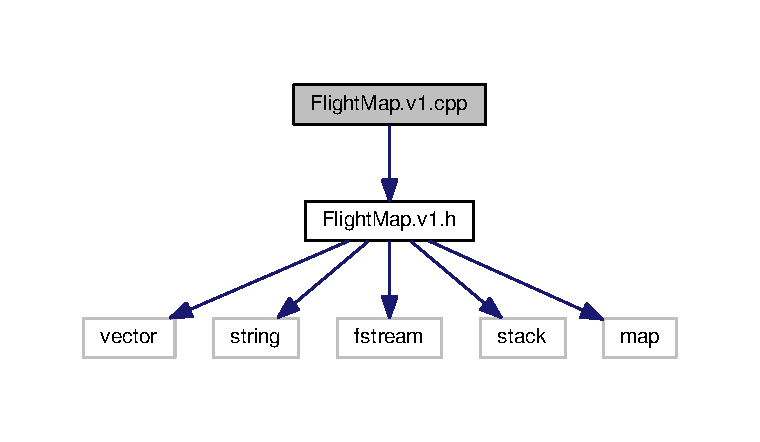
\includegraphics[width=350pt]{_flight_map_8v1_8cpp__incl}
\end{center}
\end{figure}
\subsection*{Functions}
\begin{DoxyCompactItemize}
\item 
bool \hyperlink{_flight_map_8v1_8cpp_a6b70adc00e6e8dbbadb08ee4d266a50d}{str\+In\+Vec} (const std\+::vector$<$ std\+::string $>$ \&vec, const std\+::string \&to\+Find)
\item 
void \hyperlink{_flight_map_8v1_8cpp_a9e539298d21c3b5dcb29b355a7ec33a1}{log\+Stack\+State} (const std\+::stack$<$ std\+::string $>$ \&stack, std\+::ofstream \&log)
\end{DoxyCompactItemize}


\subsection{Function Documentation}
\index{Flight\+Map.\+v1.\+cpp@{Flight\+Map.\+v1.\+cpp}!log\+Stack\+State@{log\+Stack\+State}}
\index{log\+Stack\+State@{log\+Stack\+State}!Flight\+Map.\+v1.\+cpp@{Flight\+Map.\+v1.\+cpp}}
\subsubsection[{\texorpdfstring{log\+Stack\+State(const std\+::stack$<$ std\+::string $>$ \&stack, std\+::ofstream \&log)}{logStackState(const std::stack< std::string > &stack, std::ofstream &log)}}]{\setlength{\rightskip}{0pt plus 5cm}void log\+Stack\+State (
\begin{DoxyParamCaption}
\item[{const std\+::stack$<$ std\+::string $>$ \&}]{stack, }
\item[{std\+::ofstream \&}]{log}
\end{DoxyParamCaption}
)}\hypertarget{_flight_map_8v1_8cpp_a9e539298d21c3b5dcb29b355a7ec33a1}{}\label{_flight_map_8v1_8cpp_a9e539298d21c3b5dcb29b355a7ec33a1}
\index{Flight\+Map.\+v1.\+cpp@{Flight\+Map.\+v1.\+cpp}!str\+In\+Vec@{str\+In\+Vec}}
\index{str\+In\+Vec@{str\+In\+Vec}!Flight\+Map.\+v1.\+cpp@{Flight\+Map.\+v1.\+cpp}}
\subsubsection[{\texorpdfstring{str\+In\+Vec(const std\+::vector$<$ std\+::string $>$ \&vec, const std\+::string \&to\+Find)}{strInVec(const std::vector< std::string > &vec, const std::string &toFind)}}]{\setlength{\rightskip}{0pt plus 5cm}bool str\+In\+Vec (
\begin{DoxyParamCaption}
\item[{const std\+::vector$<$ std\+::string $>$ \&}]{vec, }
\item[{const std\+::string \&}]{to\+Find}
\end{DoxyParamCaption}
)}\hypertarget{_flight_map_8v1_8cpp_a6b70adc00e6e8dbbadb08ee4d266a50d}{}\label{_flight_map_8v1_8cpp_a6b70adc00e6e8dbbadb08ee4d266a50d}

\hypertarget{_flight_map_8v1_8h}{}\section{Flight\+Map.\+v1.\+h File Reference}
\label{_flight_map_8v1_8h}\index{Flight\+Map.\+v1.\+h@{Flight\+Map.\+v1.\+h}}
{\ttfamily \#include $<$vector$>$}\\*
{\ttfamily \#include $<$string$>$}\\*
{\ttfamily \#include $<$fstream$>$}\\*
{\ttfamily \#include $<$stack$>$}\\*
{\ttfamily \#include $<$map$>$}\\*
Include dependency graph for Flight\+Map.\+v1.\+h\+:\nopagebreak
\begin{figure}[H]
\begin{center}
\leavevmode
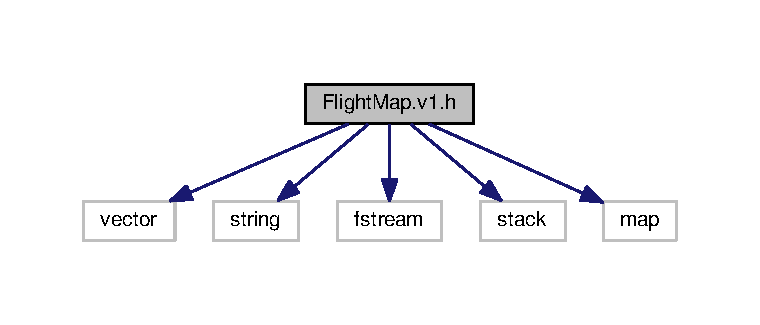
\includegraphics[width=350pt]{_flight_map_8v1_8h__incl}
\end{center}
\end{figure}
This graph shows which files directly or indirectly include this file\+:\nopagebreak
\begin{figure}[H]
\begin{center}
\leavevmode
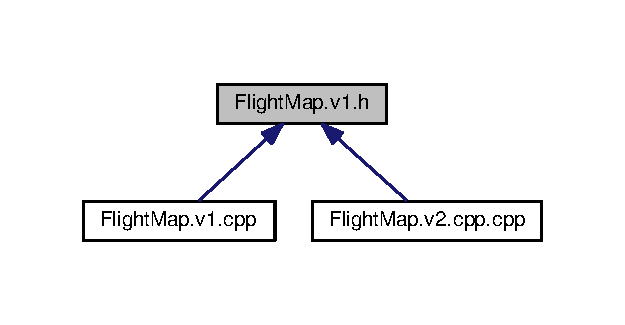
\includegraphics[width=300pt]{_flight_map_8v1_8h__dep__incl}
\end{center}
\end{figure}
\subsection*{Classes}
\begin{DoxyCompactItemize}
\item 
struct \hyperlink{struct_connection_v1}{Connection\+V1}
\begin{DoxyCompactList}\small\item\em Represents a v1 connection between cities. \end{DoxyCompactList}\item 
class \hyperlink{class_city_node_v1}{City\+Node\+V1}
\begin{DoxyCompactList}\small\item\em Represents a v1 node in the city adjacency map. \end{DoxyCompactList}\item 
class \hyperlink{class_flight_map_v1}{Flight\+Map\+V1}
\begin{DoxyCompactList}\small\item\em Represents a v1 flight map. \end{DoxyCompactList}\end{DoxyCompactItemize}

\hypertarget{_flight_map_8v2_8cpp}{}\section{Flight\+Map.\+v2.\+cpp File Reference}
\label{_flight_map_8v2_8cpp}\index{Flight\+Map.\+v2.\+cpp@{Flight\+Map.\+v2.\+cpp}}
{\ttfamily \#include \char`\"{}Flight\+Map.\+v2.\+h\char`\"{}}\\*
Include dependency graph for Flight\+Map.\+v2.\+cpp\+:
\nopagebreak
\begin{figure}[H]
\begin{center}
\leavevmode
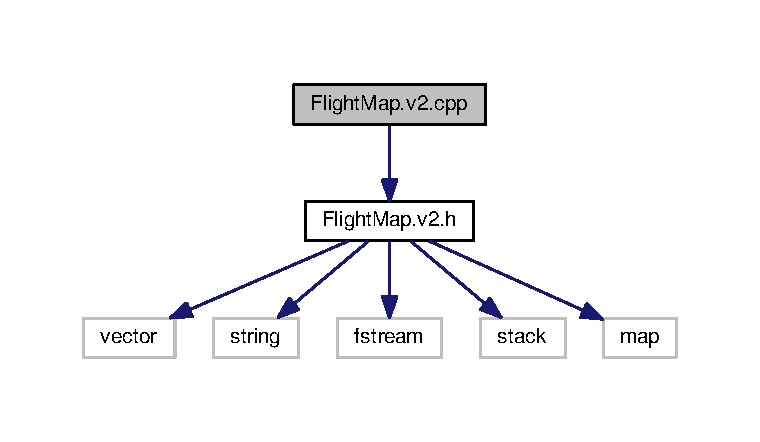
\includegraphics[width=350pt]{_flight_map_8v2_8cpp__incl}
\end{center}
\end{figure}
\subsection*{Functions}
\begin{DoxyCompactItemize}
\item 
bool \hyperlink{_flight_map_8v2_8cpp_a6b70adc00e6e8dbbadb08ee4d266a50d}{str\+In\+Vec} (const std\+::vector$<$ std\+::string $>$ \&vec, const std\+::string \&to\+Find)
\item 
void \hyperlink{_flight_map_8v2_8cpp_a9e539298d21c3b5dcb29b355a7ec33a1}{log\+Stack\+State} (const std\+::stack$<$ std\+::string $>$ \&stack, std\+::ofstream \&log)
\end{DoxyCompactItemize}


\subsection{Function Documentation}
\index{Flight\+Map.\+v2.\+cpp@{Flight\+Map.\+v2.\+cpp}!log\+Stack\+State@{log\+Stack\+State}}
\index{log\+Stack\+State@{log\+Stack\+State}!Flight\+Map.\+v2.\+cpp@{Flight\+Map.\+v2.\+cpp}}
\subsubsection[{\texorpdfstring{log\+Stack\+State(const std\+::stack$<$ std\+::string $>$ \&stack, std\+::ofstream \&log)}{logStackState(const std::stack< std::string > &stack, std::ofstream &log)}}]{\setlength{\rightskip}{0pt plus 5cm}void log\+Stack\+State (
\begin{DoxyParamCaption}
\item[{const std\+::stack$<$ std\+::string $>$ \&}]{stack, }
\item[{std\+::ofstream \&}]{log}
\end{DoxyParamCaption}
)}\hypertarget{_flight_map_8v2_8cpp_a9e539298d21c3b5dcb29b355a7ec33a1}{}\label{_flight_map_8v2_8cpp_a9e539298d21c3b5dcb29b355a7ec33a1}
\index{Flight\+Map.\+v2.\+cpp@{Flight\+Map.\+v2.\+cpp}!str\+In\+Vec@{str\+In\+Vec}}
\index{str\+In\+Vec@{str\+In\+Vec}!Flight\+Map.\+v2.\+cpp@{Flight\+Map.\+v2.\+cpp}}
\subsubsection[{\texorpdfstring{str\+In\+Vec(const std\+::vector$<$ std\+::string $>$ \&vec, const std\+::string \&to\+Find)}{strInVec(const std::vector< std::string > &vec, const std::string &toFind)}}]{\setlength{\rightskip}{0pt plus 5cm}bool str\+In\+Vec (
\begin{DoxyParamCaption}
\item[{const std\+::vector$<$ std\+::string $>$ \&}]{vec, }
\item[{const std\+::string \&}]{to\+Find}
\end{DoxyParamCaption}
)}\hypertarget{_flight_map_8v2_8cpp_a6b70adc00e6e8dbbadb08ee4d266a50d}{}\label{_flight_map_8v2_8cpp_a6b70adc00e6e8dbbadb08ee4d266a50d}

\hypertarget{_flight_map_8v2_8cpp_8cpp}{}\section{Flight\+Map.\+v2.\+cpp.\+cpp File Reference}
\label{_flight_map_8v2_8cpp_8cpp}\index{Flight\+Map.\+v2.\+cpp.\+cpp@{Flight\+Map.\+v2.\+cpp.\+cpp}}
{\ttfamily \#include \char`\"{}Flight\+Map.\+v1.\+h\char`\"{}}\\*
{\ttfamily \#include $<$iostream$>$}\\*
Include dependency graph for Flight\+Map.\+v2.\+cpp.\+cpp\+:\nopagebreak
\begin{figure}[H]
\begin{center}
\leavevmode
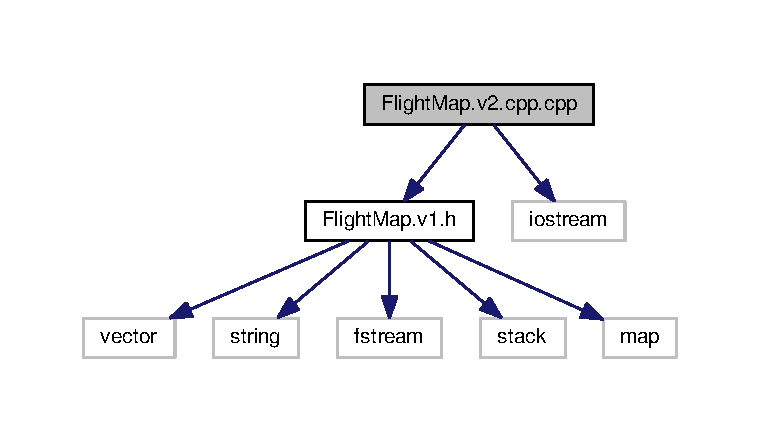
\includegraphics[width=350pt]{_flight_map_8v2_8cpp_8cpp__incl}
\end{center}
\end{figure}
\subsection*{Functions}
\begin{DoxyCompactItemize}
\item 
bool \hyperlink{_flight_map_8v2_8cpp_8cpp_a6b70adc00e6e8dbbadb08ee4d266a50d}{str\+In\+Vec} (const std\+::vector$<$ std\+::string $>$ \&vec, const std\+::string \&to\+Find)
\item 
void \hyperlink{_flight_map_8v2_8cpp_8cpp_a9e539298d21c3b5dcb29b355a7ec33a1}{log\+Stack\+State} (const std\+::stack$<$ std\+::string $>$ \&stack, std\+::ofstream \&log)
\end{DoxyCompactItemize}


\subsection{Function Documentation}
\index{Flight\+Map.\+v2.\+cpp.\+cpp@{Flight\+Map.\+v2.\+cpp.\+cpp}!log\+Stack\+State@{log\+Stack\+State}}
\index{log\+Stack\+State@{log\+Stack\+State}!Flight\+Map.\+v2.\+cpp.\+cpp@{Flight\+Map.\+v2.\+cpp.\+cpp}}
\subsubsection[{\texorpdfstring{log\+Stack\+State(const std\+::stack$<$ std\+::string $>$ \&stack, std\+::ofstream \&log)}{logStackState(const std::stack< std::string > &stack, std::ofstream &log)}}]{\setlength{\rightskip}{0pt plus 5cm}void log\+Stack\+State (
\begin{DoxyParamCaption}
\item[{const std\+::stack$<$ std\+::string $>$ \&}]{stack, }
\item[{std\+::ofstream \&}]{log}
\end{DoxyParamCaption}
)}\hypertarget{_flight_map_8v2_8cpp_8cpp_a9e539298d21c3b5dcb29b355a7ec33a1}{}\label{_flight_map_8v2_8cpp_8cpp_a9e539298d21c3b5dcb29b355a7ec33a1}
\index{Flight\+Map.\+v2.\+cpp.\+cpp@{Flight\+Map.\+v2.\+cpp.\+cpp}!str\+In\+Vec@{str\+In\+Vec}}
\index{str\+In\+Vec@{str\+In\+Vec}!Flight\+Map.\+v2.\+cpp.\+cpp@{Flight\+Map.\+v2.\+cpp.\+cpp}}
\subsubsection[{\texorpdfstring{str\+In\+Vec(const std\+::vector$<$ std\+::string $>$ \&vec, const std\+::string \&to\+Find)}{strInVec(const std::vector< std::string > &vec, const std::string &toFind)}}]{\setlength{\rightskip}{0pt plus 5cm}bool str\+In\+Vec (
\begin{DoxyParamCaption}
\item[{const std\+::vector$<$ std\+::string $>$ \&}]{vec, }
\item[{const std\+::string \&}]{to\+Find}
\end{DoxyParamCaption}
)}\hypertarget{_flight_map_8v2_8cpp_8cpp_a6b70adc00e6e8dbbadb08ee4d266a50d}{}\label{_flight_map_8v2_8cpp_8cpp_a6b70adc00e6e8dbbadb08ee4d266a50d}

\hypertarget{_flight_map_8v2_8h}{}\section{Flight\+Map.\+v2.\+h File Reference}
\label{_flight_map_8v2_8h}\index{Flight\+Map.\+v2.\+h@{Flight\+Map.\+v2.\+h}}
{\ttfamily \#include $<$vector$>$}\\*
{\ttfamily \#include $<$string$>$}\\*
{\ttfamily \#include $<$fstream$>$}\\*
{\ttfamily \#include $<$stack$>$}\\*
{\ttfamily \#include $<$map$>$}\\*
Include dependency graph for Flight\+Map.\+v2.\+h\+:\nopagebreak
\begin{figure}[H]
\begin{center}
\leavevmode
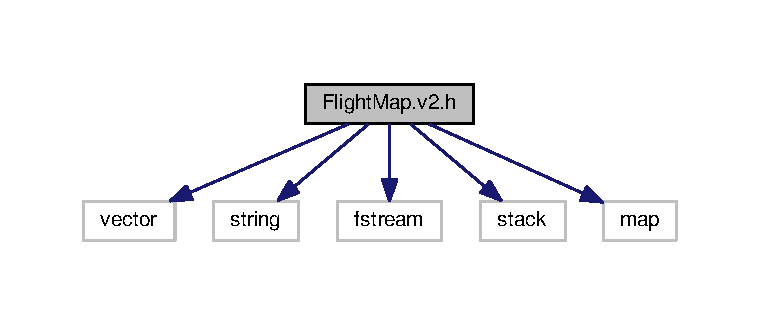
\includegraphics[width=350pt]{_flight_map_8v2_8h__incl}
\end{center}
\end{figure}
This graph shows which files directly or indirectly include this file\+:\nopagebreak
\begin{figure}[H]
\begin{center}
\leavevmode
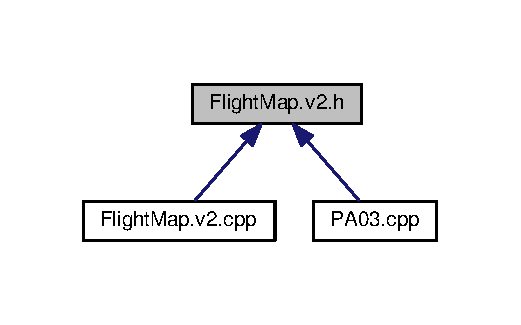
\includegraphics[width=250pt]{_flight_map_8v2_8h__dep__incl}
\end{center}
\end{figure}
\subsection*{Classes}
\begin{DoxyCompactItemize}
\item 
struct \hyperlink{struct_connection_v2}{Connection\+V2}
\begin{DoxyCompactList}\small\item\em Represents a V2 connection between cities. \end{DoxyCompactList}\item 
class \hyperlink{class_city_node_v2}{City\+Node\+V2}
\begin{DoxyCompactList}\small\item\em Represents a v2 node in the city adjacency map. \end{DoxyCompactList}\item 
class \hyperlink{class_flight_map_v2}{Flight\+Map\+V2}
\begin{DoxyCompactList}\small\item\em Represents a v2 flight map. \end{DoxyCompactList}\end{DoxyCompactItemize}

\hypertarget{_p_a03_8cpp}{}\section{P\+A03.\+cpp File Reference}
\label{_p_a03_8cpp}\index{P\+A03.\+cpp@{P\+A03.\+cpp}}
{\ttfamily \#include $<$iostream$>$}\\*
{\ttfamily \#include $<$fstream$>$}\\*
{\ttfamily \#include $<$string$>$}\\*
{\ttfamily \#include $<$vector$>$}\\*
{\ttfamily \#include $<$map$>$}\\*
{\ttfamily \#include $<$utility$>$}\\*
{\ttfamily \#include $<$sstream$>$}\\*
{\ttfamily \#include \char`\"{}Flight\+Map.\+v2.\+h\char`\"{}}\\*
Include dependency graph for P\+A03.\+cpp\+:\nopagebreak
\begin{figure}[H]
\begin{center}
\leavevmode
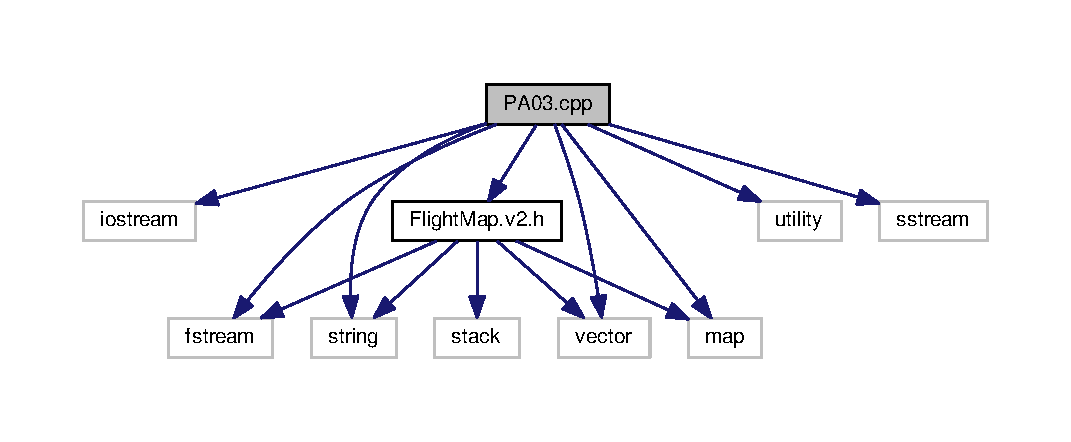
\includegraphics[width=350pt]{_p_a03_8cpp__incl}
\end{center}
\end{figure}
\subsection*{Functions}
\begin{DoxyCompactItemize}
\item 
std\+::vector$<$ std\+::string $>$ \hyperlink{_p_a03_8cpp_aacadba7e0ed37dcc51034a6bd72153f8}{split\+String} (const std\+::string \&to\+Split, char delim)
\begin{DoxyCompactList}\small\item\em Split the given string into parts by the given delimeter. \end{DoxyCompactList}\item 
int \hyperlink{_p_a03_8cpp_ab506780224ebeac7fd6b0ea2157470d3}{string\+To\+Int} (const std\+::string \&to\+Convert)
\begin{DoxyCompactList}\small\item\em Convert the given string into an int. \end{DoxyCompactList}\item 
std\+::vector$<$ std\+::string $>$ \hyperlink{_p_a03_8cpp_a3e4a5e7f9c031856621ab290e7fb20b4}{load\+Cities} (const std\+::string \&path)
\begin{DoxyCompactList}\small\item\em Load the file containing the list of cities. \end{DoxyCompactList}\item 
std\+::map$<$ std\+::pair$<$ std\+::string, std\+::string $>$, std\+::pair$<$ int, int $>$ $>$ \hyperlink{_p_a03_8cpp_a3c75582cd23f63e7c7a3743a0339ae0b}{load\+Flights} (const std\+::string \&path)
\begin{DoxyCompactList}\small\item\em Load the file containing the flight paths. \end{DoxyCompactList}\item 
std\+::vector$<$ std\+::pair$<$ std\+::string, std\+::string $>$ $>$ \hyperlink{_p_a03_8cpp_af2044c9ab5635760d4a9cb3e643dccc8}{load\+Requests} (const std\+::string \&path)
\begin{DoxyCompactList}\small\item\em Load the file containing the flight requests. \end{DoxyCompactList}\item 
int \hyperlink{_p_a03_8cpp_a3c04138a5bfe5d72780bb7e82a18e627}{main} (int argc, char $\ast$$\ast$argv)
\begin{DoxyCompactList}\small\item\em Entry point. \end{DoxyCompactList}\end{DoxyCompactItemize}


\subsection{Function Documentation}
\index{P\+A03.\+cpp@{P\+A03.\+cpp}!load\+Cities@{load\+Cities}}
\index{load\+Cities@{load\+Cities}!P\+A03.\+cpp@{P\+A03.\+cpp}}
\subsubsection[{\texorpdfstring{load\+Cities(const std\+::string \&path)}{loadCities(const std::string &path)}}]{\setlength{\rightskip}{0pt plus 5cm}std\+::vector$<$std\+::string$>$ load\+Cities (
\begin{DoxyParamCaption}
\item[{const std\+::string \&}]{path}
\end{DoxyParamCaption}
)}\hypertarget{_p_a03_8cpp_a3e4a5e7f9c031856621ab290e7fb20b4}{}\label{_p_a03_8cpp_a3e4a5e7f9c031856621ab290e7fb20b4}


Load the file containing the list of cities. 


\begin{DoxyParams}{Parameters}
{\em path} & The path to the file. \\
\hline
\end{DoxyParams}
\begin{DoxyPrecond}{Precondition}
The given path points to a readable and correctly formatted file. 
\end{DoxyPrecond}
\begin{DoxyReturn}{Returns}
A vector of all the city names read from the file. 
\end{DoxyReturn}
\index{P\+A03.\+cpp@{P\+A03.\+cpp}!load\+Flights@{load\+Flights}}
\index{load\+Flights@{load\+Flights}!P\+A03.\+cpp@{P\+A03.\+cpp}}
\subsubsection[{\texorpdfstring{load\+Flights(const std\+::string \&path)}{loadFlights(const std::string &path)}}]{\setlength{\rightskip}{0pt plus 5cm}std\+::map$<$std\+::pair$<$std\+::string, std\+::string$>$, std\+::pair$<$int, int$>$ $>$ load\+Flights (
\begin{DoxyParamCaption}
\item[{const std\+::string \&}]{path}
\end{DoxyParamCaption}
)}\hypertarget{_p_a03_8cpp_a3c75582cd23f63e7c7a3743a0339ae0b}{}\label{_p_a03_8cpp_a3c75582cd23f63e7c7a3743a0339ae0b}


Load the file containing the flight paths. 


\begin{DoxyParams}{Parameters}
{\em path} & The path to the file. \\
\hline
\end{DoxyParams}
\begin{DoxyPrecond}{Precondition}
The given path points to a readable and correctly formatted file. 
\end{DoxyPrecond}
\begin{DoxyReturn}{Returns}
A map linking string pairs (i.\+e. (\char`\"{}\+Origin\char`\"{}, \char`\"{}\+Destination\char`\"{})) to std\+::pairs of (flight number, flight cost). 
\end{DoxyReturn}
\index{P\+A03.\+cpp@{P\+A03.\+cpp}!load\+Requests@{load\+Requests}}
\index{load\+Requests@{load\+Requests}!P\+A03.\+cpp@{P\+A03.\+cpp}}
\subsubsection[{\texorpdfstring{load\+Requests(const std\+::string \&path)}{loadRequests(const std::string &path)}}]{\setlength{\rightskip}{0pt plus 5cm}std\+::vector$<$std\+::pair$<$std\+::string, std\+::string$>$ $>$ load\+Requests (
\begin{DoxyParamCaption}
\item[{const std\+::string \&}]{path}
\end{DoxyParamCaption}
)}\hypertarget{_p_a03_8cpp_af2044c9ab5635760d4a9cb3e643dccc8}{}\label{_p_a03_8cpp_af2044c9ab5635760d4a9cb3e643dccc8}


Load the file containing the flight requests. 


\begin{DoxyParams}{Parameters}
{\em path} & The path to the file. \\
\hline
\end{DoxyParams}
\begin{DoxyPrecond}{Precondition}
The given path points to a readable and correctly formatted file. 
\end{DoxyPrecond}
\begin{DoxyReturn}{Returns}
A vector containing (\char`\"{}\+Origin\char`\"{}, \char`\"{}\+Destination\char`\"{}) pairs. 
\end{DoxyReturn}
\index{P\+A03.\+cpp@{P\+A03.\+cpp}!main@{main}}
\index{main@{main}!P\+A03.\+cpp@{P\+A03.\+cpp}}
\subsubsection[{\texorpdfstring{main(int argc, char $\ast$$\ast$argv)}{main(int argc, char **argv)}}]{\setlength{\rightskip}{0pt plus 5cm}int main (
\begin{DoxyParamCaption}
\item[{int}]{argc, }
\item[{char $\ast$$\ast$}]{argv}
\end{DoxyParamCaption}
)}\hypertarget{_p_a03_8cpp_a3c04138a5bfe5d72780bb7e82a18e627}{}\label{_p_a03_8cpp_a3c04138a5bfe5d72780bb7e82a18e627}


Entry point. 

\index{P\+A03.\+cpp@{P\+A03.\+cpp}!split\+String@{split\+String}}
\index{split\+String@{split\+String}!P\+A03.\+cpp@{P\+A03.\+cpp}}
\subsubsection[{\texorpdfstring{split\+String(const std\+::string \&to\+Split, char delim)}{splitString(const std::string &toSplit, char delim)}}]{\setlength{\rightskip}{0pt plus 5cm}std\+::vector$<$std\+::string$>$ split\+String (
\begin{DoxyParamCaption}
\item[{const std\+::string \&}]{to\+Split, }
\item[{char}]{delim}
\end{DoxyParamCaption}
)}\hypertarget{_p_a03_8cpp_aacadba7e0ed37dcc51034a6bd72153f8}{}\label{_p_a03_8cpp_aacadba7e0ed37dcc51034a6bd72153f8}


Split the given string into parts by the given delimeter. 


\begin{DoxyParams}{Parameters}
{\em to\+Split} & The string to split. \\
\hline
{\em delim} & The delimeter. \\
\hline
\end{DoxyParams}
\begin{DoxyReturn}{Returns}
A vector containing the parts of the string. 
\end{DoxyReturn}
\index{P\+A03.\+cpp@{P\+A03.\+cpp}!string\+To\+Int@{string\+To\+Int}}
\index{string\+To\+Int@{string\+To\+Int}!P\+A03.\+cpp@{P\+A03.\+cpp}}
\subsubsection[{\texorpdfstring{string\+To\+Int(const std\+::string \&to\+Convert)}{stringToInt(const std::string &toConvert)}}]{\setlength{\rightskip}{0pt plus 5cm}int string\+To\+Int (
\begin{DoxyParamCaption}
\item[{const std\+::string \&}]{to\+Convert}
\end{DoxyParamCaption}
)}\hypertarget{_p_a03_8cpp_ab506780224ebeac7fd6b0ea2157470d3}{}\label{_p_a03_8cpp_ab506780224ebeac7fd6b0ea2157470d3}


Convert the given string into an int. 


\begin{DoxyParams}{Parameters}
{\em to\+Convert} & The string to convert. \\
\hline
\end{DoxyParams}
\begin{DoxyPrecond}{Precondition}
The given string can be converted into an integer. 
\end{DoxyPrecond}
\begin{DoxyReturn}{Returns}
The int value read fromt the given string. 
\end{DoxyReturn}

%--- End generated contents ---

% Index
\backmatter
\newpage
\phantomsection
\clearemptydoublepage
\addcontentsline{toc}{chapter}{Index}
\printindex

\end{document}
